\subsection{Velocità della luce}

Si vuole utilizzare l'apparato a disposizione per misurare la velocità della luce. Si noti che con tale apparato è possibile misurare solamente differenze di tempi
e non tempi assoluti (vista tutta l'elettronica utilizzata). Le misure sono state prese come descritto nell'analisi dati, e a disposizione quindi si hanno:
\begin{itemize}
\item la distanza tra i due rivelatori
\item i diversi ritardi nella rivelazione nelle due diverse configurazioni
\item le dimensioni del piombo contenente la sorgente
\item il datasheet dei rivelatori
\end{itemize}
Si cerchi una formula per ricavare la velocità della luce date queste informazioni. Il ragionamento farà uso di due approssimazioni: la sorgente è puntiforme lungo la direzione
di volo dei fotoni rivelati (assumibile in quanto consisteva in un disco posto in maniera perpendicolare a tale direzione)
e si può pensare il fotone venga rivelato sempre nella stessa posizione dentro il rivelatore.\\

Con tali ipotesi, si considerino le misure di lunghezze con la seguente notazione:
\begin{itemize}
\item $R_1$ indica lo spazio medio percorso dai fotoni nel rivelatore prima di interagire con lo stesso
\item $x_1$ indica la distanza tra la placca in piombo più vicina e il rivelatore 1
\item $\delta_1$ indica lo spessore della placca in piombo più vicina al rivelatore 1
\end{itemize}
E analoga notazione per quanto riguarda il rivelatore 2. In poche parole le ipotesi fatte consistono nel fatto che i valori di $R_1$ $R_2$ si possono prendere
come esatti.\footnote{In realtà, questa ipotesi viene verificata nel limite delle infinite misure; dato che il campione preso è sufficientemente grande, si suppone essa sia
valida}, mentre l'ipotesi di sorgente puntiforme è necessaria per ridurre il problema in tre dimensioni a un problema unidimensionale.\\
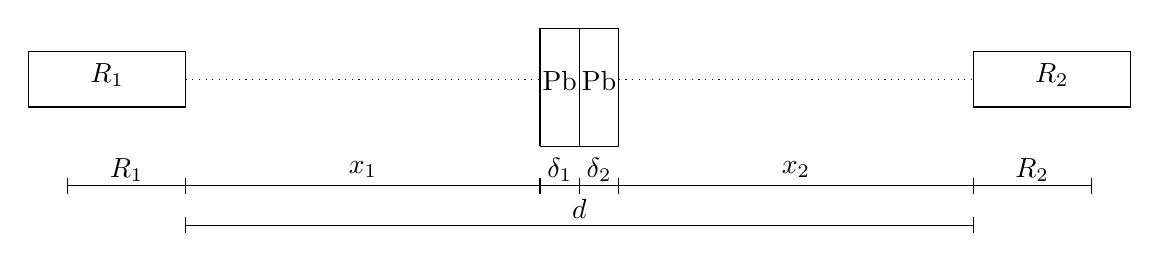
\begin{tikzpicture}
%\draw[->,thick] (-4,0)--(4,0) node[right]{$z$};

%\node [label=below:-e,draw,fill=black,circle,inner sep=0pt,minimum size=3pt] at (-3,0) {};
%\node [label=below:+e,draw,fill=black,circle,inner sep=0pt,minimum size=3pt] at (-2,0) {};
%\node [label=below:+e,draw,fill=black,circle,inner sep=0pt,minimum size=3pt] at (2,0) {};
%\node [label=below:-e,draw,fill=black,circle,inner sep=0pt,minimum size=3pt] at (3,0) {};


\draw[] (-4,0)--(-4,0.7)--(-2,0.7)--(-2,0)--(-4,0) node[label=above:$R_1$, black, midway, yshift=0.3]{}; %primo rivelatore
\draw[] (8,0)--(8,0.7)--(10,0.7)--(10,0)--(8,0) node[label=above:$R_2$, black, midway, yshift=0.3]{}; %secondo rivelatore

\draw[] (2.5,-0.5)--(2.5,1)--(3,1)--(3,-0.5)--(2.5,-0.5) node[label=above:Pb, black, midway, yshift=13]{}; %primo piombo
\draw[] (3,-0.5)--(3,1)--(3.5,1)--(3.5,-0.5)--(3,-0.5) node[label=above:Pb, black, midway, yshift=13]{}; %secondo piombo

%\node[starburst, minimum width=3cm, minimum height=2cm,line width=1.5pt]{};

\draw[] (-3.5,-1)--(9.5,-1) node[right]{};

\draw[] (-3.5,-1.1)--(-3.5,-0.9){};
\draw[] (-2,-1.1)--(-2,-0.9){};
\draw[] (2.5,-1.1)--(2.5,-0.9){};
\draw[] (3,-1.1)--(3,-0.9){};
\draw[] (3.5,-1.1)--(3.5,-0.9){};
\draw[] (8,-1.1)--(8,-0.9){};
\draw[] (9.5,-1.1)--(9.5,-0.9){};

\node[] at (-2.75,-0.8) {$R_1$};
\node[] at (0.25,-0.8) {$x_1$};
\node[] at (2.75,-0.8) {$\delta_1$};
\node[] at (3.25,-0.8) {$\delta_2$};
\node[] at (5.75,-0.8) {$x_2$};
\node[] at (8.75,-0.8) {$R_2$};

\draw[dotted](-2,0.35)--(2.5,0.35){};
\draw[dotted](3.5,0.35)--(8,0.35){};

\draw[] (-2,-1.5)--(8,-1.5) node[right]{};
\node[] at (3,-1.3) {$d$};
\draw[] (-2,-1.6)--(-2,-1.4){};
\draw[] (8,-1.6)--(8,-1.4){};


%\draw [decorate,decoration={brace,amplitude=10pt},xshift=0pt,yshift=0pt] (-3,0) -- (-2,0) node [label=above:$z_2$,black,midway,yshift=0.2cm] {};
%\draw [decorate,decoration={brace,amplitude=10pt},xshift=0pt,yshift=0pt] (-2,0) -- (2,0) node [label=above:$R$,black,midway,yshift=0.2cm] {};
%\draw [decorate,decoration={brace,amplitude=10pt},xshift=0pt,yshift=0pt] (2,0) -- (3,0) node [label=above:$z_1$,black,midway,yshift=0.2cm] {};

\end{tikzpicture} 


A questo punto, se la configurazione è la A, si possono descrivere i tempi di percorrenza dei fotoni prima che vengano rivelati come:
$$
  t_{1A} = \frac{\delta_1 + nR_1}{c} \hspace{2cm} t_{2A} = \frac{\delta_2 + x_2 + nR_2}{c}
$$
Ove $n$ indica un eventuale coefficiente di rifrazione all'interno del rivelatore stesso. Quindi il TAC rivelerà l'intervallo temporale:
$$
  \delta t_A = t_{2A} - t_{1A} = \frac{\delta_2 + x_2 + nR_2-\delta_1-nR_1}{c}
$$
Analogamente per la configurazione B si trova:
$$
  t_{1B} = \frac{\delta_1 + x_1 + nR_1}{c} \hspace{2cm} t_{2B} = \frac{\delta_2 + nR_2}{c}
$$
e l'intervallo rilevato dal TAC sarà:
$$
  \Delta t_B = t_{2B} - t_{1B} = \frac{\delta_2 + nR_2 - \delta_1 - x_1 - nR_1}{c}
$$
A questo punto, però, questi due intervalli non hanno senso presi singolarmente, in quanto non rivelano effettivamente un intervallo temporale ma il tempo riferito ad
uno zero che, sebbene non sia noto oggettivamente, è lo stesso per entrambe le misure (infatti non si è toccato l'apparato strumentale se non per spostare la sorgente
racchiusa tra le placche di piombo). Perciò ha senso fisico la loro differenza, che si può stimare con facilità:
$$
  \Delta t = \Delta t_A - \Delta t_B = \frac{{\delta_2 + x_2 + nR_2 - \delta_1 - nR_1}{-\delta_2 - nR_2 + \delta_1 + x_1 + nR_1}}{c} = \frac{x_1 + x_2}{c}
$$
Perciò per stimare la velocità della luce è sufficiente andare a misurare la distanza dei due rivelatori a meno delle placche di piombo e la distanza temporale tra i due
picchi nei grafici calibrati del TAC. Però, in sede di esecuzione dell'esperimento, non si è effettivamente misurata quella distanza ma solamente le distanze tra la sorgente
e i rivelatori nelle due configurazioni, quindi si ha una stima di $\delta$ e una stima di $ 2 \delta + x$ per i due casi.\\

Si venga alla vera e propria analisi dati: si vuole applicare la formula, appena dimostrata:
$$
  c = \frac{x_1+x_2}{\Delta t}
$$
si ragioni sul numeratore, cioè la misura di lunghezza: si conoscono i valori, misurati con il metro:
$$
  d = 173.2 cm \hspace{2cm} \delta = 3.7 cm
$$
ove d indica la distanza tra i due rivelatori e $\delta$ indica le misure (uguali) dei blocchi di piombo.
Ora si è interessati a $x_1+x_2$, per motivi geometrici si può riscrivere in funzione delle variabili misurate come:
$$
  x_1+x_2 = 2 ( d - 2 \delta)
$$
Come errore sulle variabili si considera un errore triangolare associato al fatto che il metro aveva una scala dei millimetri, quindi si ha
$$
  \sigma_d = \sigma_\delta = \frac{0.5\text{mm}}{\sqrt6} = 0.2 mm
$$
\\

Ora si pensi al denominatore dell'equazione per la velocità della luce, cioè la differenza tra le distanze temporali nelle due diverse configurazioni dell'esperimento.
Si riscriva tenendo conto della calibrazione:
$$
  \Delta t = \Delta t_A - \Delta t_B = m\Delta t_A + q - m\Delta t_B - q = m (\Delta t_A - \Delta t_B) 
$$
Ove $m,q$, sono i coefficienti della calibrazione stimati nelle sezioni precedenti. I due picchi si possono vedere, già calibrati, nella figura sottostante.\\
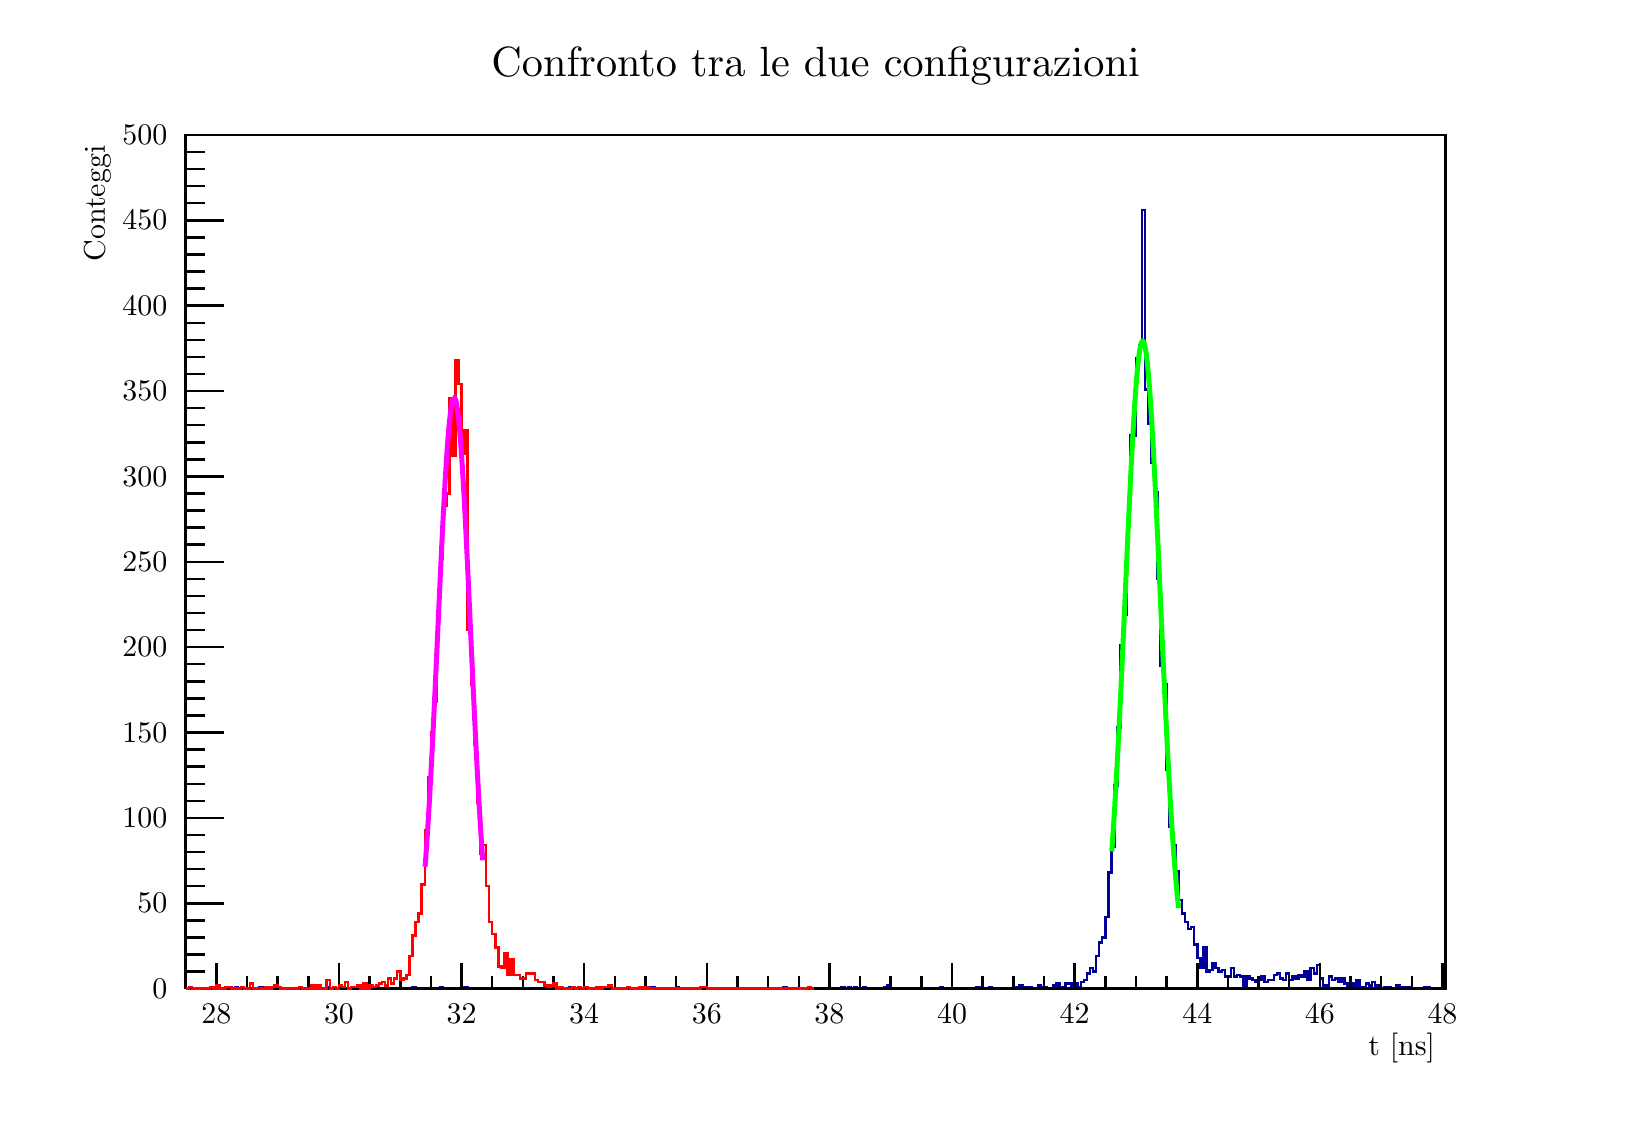
\begin{tikzpicture}
\pgfdeclareplotmark{cross} {
\pgfpathmoveto{\pgfpoint{-0.3\pgfplotmarksize}{\pgfplotmarksize}}
\pgfpathlineto{\pgfpoint{+0.3\pgfplotmarksize}{\pgfplotmarksize}}
\pgfpathlineto{\pgfpoint{+0.3\pgfplotmarksize}{0.3\pgfplotmarksize}}
\pgfpathlineto{\pgfpoint{+1\pgfplotmarksize}{0.3\pgfplotmarksize}}
\pgfpathlineto{\pgfpoint{+1\pgfplotmarksize}{-0.3\pgfplotmarksize}}
\pgfpathlineto{\pgfpoint{+0.3\pgfplotmarksize}{-0.3\pgfplotmarksize}}
\pgfpathlineto{\pgfpoint{+0.3\pgfplotmarksize}{-1.\pgfplotmarksize}}
\pgfpathlineto{\pgfpoint{-0.3\pgfplotmarksize}{-1.\pgfplotmarksize}}
\pgfpathlineto{\pgfpoint{-0.3\pgfplotmarksize}{-0.3\pgfplotmarksize}}
\pgfpathlineto{\pgfpoint{-1.\pgfplotmarksize}{-0.3\pgfplotmarksize}}
\pgfpathlineto{\pgfpoint{-1.\pgfplotmarksize}{0.3\pgfplotmarksize}}
\pgfpathlineto{\pgfpoint{-0.3\pgfplotmarksize}{0.3\pgfplotmarksize}}
\pgfpathclose
\pgfusepathqstroke
}
\pgfdeclareplotmark{cross*} {
\pgfpathmoveto{\pgfpoint{-0.3\pgfplotmarksize}{\pgfplotmarksize}}
\pgfpathlineto{\pgfpoint{+0.3\pgfplotmarksize}{\pgfplotmarksize}}
\pgfpathlineto{\pgfpoint{+0.3\pgfplotmarksize}{0.3\pgfplotmarksize}}
\pgfpathlineto{\pgfpoint{+1\pgfplotmarksize}{0.3\pgfplotmarksize}}
\pgfpathlineto{\pgfpoint{+1\pgfplotmarksize}{-0.3\pgfplotmarksize}}
\pgfpathlineto{\pgfpoint{+0.3\pgfplotmarksize}{-0.3\pgfplotmarksize}}
\pgfpathlineto{\pgfpoint{+0.3\pgfplotmarksize}{-1.\pgfplotmarksize}}
\pgfpathlineto{\pgfpoint{-0.3\pgfplotmarksize}{-1.\pgfplotmarksize}}
\pgfpathlineto{\pgfpoint{-0.3\pgfplotmarksize}{-0.3\pgfplotmarksize}}
\pgfpathlineto{\pgfpoint{-1.\pgfplotmarksize}{-0.3\pgfplotmarksize}}
\pgfpathlineto{\pgfpoint{-1.\pgfplotmarksize}{0.3\pgfplotmarksize}}
\pgfpathlineto{\pgfpoint{-0.3\pgfplotmarksize}{0.3\pgfplotmarksize}}
\pgfpathclose
\pgfusepathqfillstroke
}
\pgfdeclareplotmark{newstar} {
\pgfpathmoveto{\pgfqpoint{0pt}{\pgfplotmarksize}}
\pgfpathlineto{\pgfqpointpolar{44}{0.5\pgfplotmarksize}}
\pgfpathlineto{\pgfqpointpolar{18}{\pgfplotmarksize}}
\pgfpathlineto{\pgfqpointpolar{-20}{0.5\pgfplotmarksize}}
\pgfpathlineto{\pgfqpointpolar{-54}{\pgfplotmarksize}}
\pgfpathlineto{\pgfqpointpolar{-90}{0.5\pgfplotmarksize}}
\pgfpathlineto{\pgfqpointpolar{234}{\pgfplotmarksize}}
\pgfpathlineto{\pgfqpointpolar{198}{0.5\pgfplotmarksize}}
\pgfpathlineto{\pgfqpointpolar{162}{\pgfplotmarksize}}
\pgfpathlineto{\pgfqpointpolar{134}{0.5\pgfplotmarksize}}
\pgfpathclose
\pgfusepathqstroke
}
\pgfdeclareplotmark{newstar*} {
\pgfpathmoveto{\pgfqpoint{0pt}{\pgfplotmarksize}}
\pgfpathlineto{\pgfqpointpolar{44}{0.5\pgfplotmarksize}}
\pgfpathlineto{\pgfqpointpolar{18}{\pgfplotmarksize}}
\pgfpathlineto{\pgfqpointpolar{-20}{0.5\pgfplotmarksize}}
\pgfpathlineto{\pgfqpointpolar{-54}{\pgfplotmarksize}}
\pgfpathlineto{\pgfqpointpolar{-90}{0.5\pgfplotmarksize}}
\pgfpathlineto{\pgfqpointpolar{234}{\pgfplotmarksize}}
\pgfpathlineto{\pgfqpointpolar{198}{0.5\pgfplotmarksize}}
\pgfpathlineto{\pgfqpointpolar{162}{\pgfplotmarksize}}
\pgfpathlineto{\pgfqpointpolar{134}{0.5\pgfplotmarksize}}
\pgfpathclose
\pgfusepathqfillstroke
}
\definecolor{c}{rgb}{1,1,1};
\draw [color=c, fill=c] (0,0) rectangle (20,13.553);
\draw [color=c, fill=c] (2,1.3553) rectangle (18,12.1977);
\definecolor{c}{rgb}{0,0,0};
\draw [c,line width=0.9] (2,1.3553) -- (2,12.1977) -- (18,12.1977) -- (18,1.3553) -- (2,1.3553);
\definecolor{c}{rgb}{1,1,1};
\draw [color=c, fill=c] (2,1.3553) rectangle (18,12.1977);
\definecolor{c}{rgb}{0,0,0};
\draw [c,line width=0.9] (2,1.3553) -- (2,12.1977) -- (18,12.1977) -- (18,1.3553) -- (2,1.3553);
\definecolor{c}{rgb}{0,0,0.6};
\draw [c,line width=0.9] (2,1.3553) -- (2.03893,1.3553) -- (2.03893,1.3553) -- (2.07786,1.3553) -- (2.07786,1.3553) -- (2.11679,1.3553) -- (2.11679,1.3553) -- (2.15572,1.3553) -- (2.15572,1.3553) -- (2.19465,1.3553) -- (2.19465,1.3553) --
 (2.23358,1.3553) -- (2.23358,1.3553) -- (2.27251,1.3553) -- (2.27251,1.3553) -- (2.31144,1.3553) -- (2.31144,1.3553) -- (2.35037,1.3553) -- (2.35037,1.3553) -- (2.38929,1.3553) -- (2.38929,1.3553) -- (2.42822,1.3553) -- (2.42822,1.3553) --
 (2.46715,1.3553) -- (2.46715,1.3553) -- (2.50608,1.3553) -- (2.50608,1.3553) -- (2.54501,1.3553) -- (2.54501,1.3553) -- (2.58394,1.3553) -- (2.58394,1.3553) -- (2.62287,1.3553) -- (2.62287,1.37699) -- (2.6618,1.37699) -- (2.6618,1.3553) --
 (2.70073,1.3553) -- (2.70073,1.37699) -- (2.73966,1.37699) -- (2.73966,1.3553) -- (2.77859,1.3553) -- (2.77859,1.3553) -- (2.81752,1.3553) -- (2.81752,1.3553) -- (2.85645,1.3553) -- (2.85645,1.3553) -- (2.89538,1.3553) -- (2.89538,1.3553) --
 (2.93431,1.3553) -- (2.93431,1.37699) -- (2.97324,1.37699) -- (2.97324,1.3553) -- (3.01217,1.3553) -- (3.01217,1.3553) -- (3.0511,1.3553) -- (3.0511,1.3553) -- (3.09002,1.3553) -- (3.09002,1.3553) -- (3.12895,1.3553) -- (3.12895,1.3553) --
 (3.16788,1.3553) -- (3.16788,1.3553) -- (3.20681,1.3553) -- (3.20681,1.3553) -- (3.24574,1.3553) -- (3.24574,1.3553) -- (3.28467,1.3553) -- (3.28467,1.3553) -- (3.3236,1.3553) -- (3.3236,1.3553) -- (3.36253,1.3553) -- (3.36253,1.3553) --
 (3.40146,1.3553) -- (3.40146,1.3553) -- (3.44039,1.3553) -- (3.44039,1.3553) -- (3.47932,1.3553) -- (3.47932,1.3553) -- (3.51825,1.3553) -- (3.51825,1.3553) -- (3.55718,1.3553) -- (3.55718,1.3553) -- (3.59611,1.3553) -- (3.59611,1.3553) --
 (3.63504,1.3553) -- (3.63504,1.3553) -- (3.67397,1.3553) -- (3.67397,1.3553) -- (3.7129,1.3553) -- (3.7129,1.3553) -- (3.75182,1.3553) -- (3.75182,1.3553) -- (3.79075,1.3553) -- (3.79075,1.37699) -- (3.82968,1.37699) -- (3.82968,1.3553) --
 (3.86861,1.3553) -- (3.86861,1.3553) -- (3.90754,1.3553) -- (3.90754,1.3553) -- (3.94647,1.3553) -- (3.94647,1.3553) -- (3.9854,1.3553) -- (3.9854,1.3553) -- (4.02433,1.3553) -- (4.02433,1.3553) -- (4.06326,1.3553) -- (4.06326,1.3553) --
 (4.10219,1.3553) -- (4.10219,1.3553) -- (4.14112,1.3553) -- (4.14112,1.3553) -- (4.18005,1.3553) -- (4.18005,1.3553) -- (4.21898,1.3553) -- (4.21898,1.3553) -- (4.25791,1.3553) -- (4.25791,1.3553) -- (4.29684,1.3553) -- (4.29684,1.3553) --
 (4.33577,1.3553) -- (4.33577,1.3553) -- (4.3747,1.3553) -- (4.3747,1.3553) -- (4.41363,1.3553) -- (4.41363,1.3553) -- (4.45255,1.3553) -- (4.45255,1.3553) -- (4.49148,1.3553) -- (4.49148,1.3553) -- (4.53041,1.3553) -- (4.53041,1.3553) --
 (4.56934,1.3553) -- (4.56934,1.3553) -- (4.60827,1.3553) -- (4.60827,1.3553) -- (4.6472,1.3553) -- (4.6472,1.3553) -- (4.68613,1.3553) -- (4.68613,1.3553) -- (4.72506,1.3553) -- (4.72506,1.3553) -- (4.76399,1.3553) -- (4.76399,1.3553) --
 (4.80292,1.3553) -- (4.80292,1.3553) -- (4.84185,1.3553) -- (4.84185,1.3553) -- (4.88078,1.3553) -- (4.88078,1.37699) -- (4.91971,1.37699) -- (4.91971,1.3553) -- (4.95864,1.3553) -- (4.95864,1.3553) -- (4.99757,1.3553) -- (4.99757,1.3553) --
 (5.0365,1.3553) -- (5.0365,1.3553) -- (5.07543,1.3553) -- (5.07543,1.3553) -- (5.11436,1.3553) -- (5.11436,1.3553) -- (5.15328,1.3553) -- (5.15328,1.3553) -- (5.19221,1.3553) -- (5.19221,1.3553) -- (5.23114,1.3553) -- (5.23114,1.37699) --
 (5.27007,1.37699) -- (5.27007,1.3553) -- (5.309,1.3553) -- (5.309,1.3553) -- (5.34793,1.3553) -- (5.34793,1.3553) -- (5.38686,1.3553) -- (5.38686,1.3553) -- (5.42579,1.3553) -- (5.42579,1.3553) -- (5.46472,1.3553) -- (5.46472,1.3553) --
 (5.50365,1.3553) -- (5.50365,1.37699) -- (5.54258,1.37699) -- (5.54258,1.37699) -- (5.58151,1.37699) -- (5.58151,1.3553) -- (5.62044,1.3553) -- (5.62044,1.3553) -- (5.65937,1.3553) -- (5.65937,1.3553) -- (5.6983,1.3553) -- (5.6983,1.3553) --
 (5.73723,1.3553) -- (5.73723,1.3553) -- (5.77616,1.3553) -- (5.77616,1.3553) -- (5.81509,1.3553) -- (5.81509,1.3553) -- (5.85401,1.3553) -- (5.85401,1.3553) -- (5.89294,1.3553) -- (5.89294,1.3553) -- (5.93187,1.3553) -- (5.93187,1.3553) --
 (5.9708,1.3553) -- (5.9708,1.3553) -- (6.00973,1.3553) -- (6.00973,1.3553) -- (6.04866,1.3553) -- (6.04866,1.3553) -- (6.08759,1.3553) -- (6.08759,1.3553) -- (6.12652,1.3553) -- (6.12652,1.3553) -- (6.16545,1.3553) -- (6.16545,1.3553) --
 (6.20438,1.3553) -- (6.20438,1.3553) -- (6.24331,1.3553) -- (6.24331,1.3553) -- (6.28224,1.3553) -- (6.28224,1.3553) -- (6.32117,1.3553) -- (6.32117,1.3553) -- (6.3601,1.3553) -- (6.3601,1.3553) -- (6.39903,1.3553) -- (6.39903,1.3553) --
 (6.43796,1.3553) -- (6.43796,1.3553) -- (6.47689,1.3553) -- (6.47689,1.3553) -- (6.51582,1.3553) -- (6.51582,1.3553) -- (6.55474,1.3553) -- (6.55474,1.3553) -- (6.59367,1.3553) -- (6.59367,1.3553) -- (6.6326,1.3553) -- (6.6326,1.3553) --
 (6.67153,1.3553) -- (6.67153,1.3553) -- (6.71046,1.3553) -- (6.71046,1.3553) -- (6.74939,1.3553) -- (6.74939,1.3553) -- (6.78832,1.3553) -- (6.78832,1.3553) -- (6.82725,1.3553) -- (6.82725,1.3553) -- (6.86618,1.3553) -- (6.86618,1.37699) --
 (6.90511,1.37699) -- (6.90511,1.3553) -- (6.94404,1.3553) -- (6.94404,1.3553) -- (6.98297,1.3553) -- (6.98297,1.3553) -- (7.0219,1.3553) -- (7.0219,1.3553) -- (7.06083,1.3553) -- (7.06083,1.3553) -- (7.09976,1.3553) -- (7.09976,1.3553) --
 (7.13869,1.3553) -- (7.13869,1.3553) -- (7.17762,1.3553) -- (7.17762,1.3553) -- (7.21655,1.3553) -- (7.21655,1.3553) -- (7.25547,1.3553) -- (7.25547,1.37699) -- (7.2944,1.37699) -- (7.2944,1.3553) -- (7.33333,1.3553) -- (7.33333,1.3553) --
 (7.37226,1.3553) -- (7.37226,1.3553) -- (7.41119,1.3553) -- (7.41119,1.3553) -- (7.45012,1.3553) -- (7.45012,1.3553) -- (7.48905,1.3553) -- (7.48905,1.3553) -- (7.52798,1.3553) -- (7.52798,1.3553) -- (7.56691,1.3553) -- (7.56691,1.3553) --
 (7.60584,1.3553) -- (7.60584,1.3553) -- (7.64477,1.3553) -- (7.64477,1.3553) -- (7.6837,1.3553) -- (7.6837,1.3553) -- (7.72263,1.3553) -- (7.72263,1.3553) -- (7.76156,1.3553) -- (7.76156,1.3553) -- (7.80049,1.3553) -- (7.80049,1.3553) --
 (7.83942,1.3553) -- (7.83942,1.3553) -- (7.87835,1.3553) -- (7.87835,1.3553) -- (7.91727,1.3553) -- (7.91727,1.37699) -- (7.9562,1.37699) -- (7.9562,1.3553) -- (7.99513,1.3553) -- (7.99513,1.3553) -- (8.03406,1.3553) -- (8.03406,1.3553) --
 (8.07299,1.3553) -- (8.07299,1.3553) -- (8.11192,1.3553) -- (8.11192,1.3553) -- (8.15085,1.3553) -- (8.15085,1.3553) -- (8.18978,1.3553) -- (8.18978,1.3553) -- (8.22871,1.3553) -- (8.22871,1.37699) -- (8.26764,1.37699) -- (8.26764,1.3553) --
 (8.30657,1.3553) -- (8.30657,1.3553) -- (8.3455,1.3553) -- (8.3455,1.3553) -- (8.38443,1.3553) -- (8.38443,1.3553) -- (8.42336,1.3553) -- (8.42336,1.3553) -- (8.46229,1.3553) -- (8.46229,1.3553) -- (8.50122,1.3553) -- (8.50122,1.3553) --
 (8.54015,1.3553) -- (8.54015,1.37699) -- (8.57908,1.37699) -- (8.57908,1.3553) -- (8.618,1.3553) -- (8.618,1.3553) -- (8.65693,1.3553) -- (8.65693,1.3553) -- (8.69586,1.3553) -- (8.69586,1.3553) -- (8.73479,1.3553) -- (8.73479,1.3553) --
 (8.77372,1.3553) -- (8.77372,1.3553) -- (8.81265,1.3553) -- (8.81265,1.3553) -- (8.85158,1.3553) -- (8.85158,1.3553) -- (8.89051,1.3553) -- (8.89051,1.3553) -- (8.92944,1.3553) -- (8.92944,1.3553) -- (8.96837,1.3553) -- (8.96837,1.3553) --
 (9.0073,1.3553) -- (9.0073,1.3553) -- (9.04623,1.3553) -- (9.04623,1.3553) -- (9.08516,1.3553) -- (9.08516,1.3553) -- (9.12409,1.3553) -- (9.12409,1.3553) -- (9.16302,1.3553) -- (9.16302,1.3553) -- (9.20195,1.3553) -- (9.20195,1.3553) --
 (9.24088,1.3553) -- (9.24088,1.3553) -- (9.27981,1.3553) -- (9.27981,1.3553) -- (9.31874,1.3553) -- (9.31874,1.3553) -- (9.35766,1.3553) -- (9.35766,1.3553) -- (9.39659,1.3553) -- (9.39659,1.3553) -- (9.43552,1.3553) -- (9.43552,1.3553) --
 (9.47445,1.3553) -- (9.47445,1.3553) -- (9.51338,1.3553) -- (9.51338,1.3553) -- (9.55231,1.3553) -- (9.55231,1.3553) -- (9.59124,1.3553) -- (9.59124,1.37699) -- (9.63017,1.37699) -- (9.63017,1.3553) -- (9.6691,1.3553) -- (9.6691,1.3553) --
 (9.70803,1.3553) -- (9.70803,1.3553) -- (9.74696,1.3553) -- (9.74696,1.3553) -- (9.78589,1.3553) -- (9.78589,1.3553) -- (9.82482,1.3553) -- (9.82482,1.3553) -- (9.86375,1.3553) -- (9.86375,1.3553) -- (9.90268,1.3553) -- (9.90268,1.3553) --
 (9.94161,1.3553) -- (9.94161,1.3553) -- (9.98054,1.3553) -- (9.98054,1.3553) -- (10.0195,1.3553) -- (10.0195,1.3553) -- (10.0584,1.3553) -- (10.0584,1.3553) -- (10.0973,1.3553) -- (10.0973,1.3553) -- (10.1363,1.3553) -- (10.1363,1.3553) --
 (10.1752,1.3553) -- (10.1752,1.3553) -- (10.2141,1.3553) -- (10.2141,1.3553) -- (10.253,1.3553) -- (10.253,1.3553) -- (10.292,1.3553) -- (10.292,1.3553) -- (10.3309,1.3553) -- (10.3309,1.37699) -- (10.3698,1.37699) -- (10.3698,1.3553) --
 (10.4088,1.3553) -- (10.4088,1.37699) -- (10.4477,1.37699) -- (10.4477,1.3553) -- (10.4866,1.3553) -- (10.4866,1.37699) -- (10.5255,1.37699) -- (10.5255,1.3553) -- (10.5645,1.3553) -- (10.5645,1.3553) -- (10.6034,1.3553) -- (10.6034,1.37699) --
 (10.6423,1.37699) -- (10.6423,1.3553) -- (10.6813,1.3553) -- (10.6813,1.3553) -- (10.7202,1.3553) -- (10.7202,1.3553) -- (10.7591,1.3553) -- (10.7591,1.3553) -- (10.7981,1.3553) -- (10.7981,1.3553) -- (10.837,1.3553) -- (10.837,1.3553) --
 (10.8759,1.3553) -- (10.8759,1.37699) -- (10.9148,1.37699) -- (10.9148,1.39867) -- (10.9538,1.39867) -- (10.9538,1.3553) -- (10.9927,1.3553) -- (10.9927,1.3553) -- (11.0316,1.3553) -- (11.0316,1.3553) -- (11.0706,1.3553) -- (11.0706,1.3553) --
 (11.1095,1.3553) -- (11.1095,1.3553) -- (11.1484,1.3553) -- (11.1484,1.3553) -- (11.1873,1.3553) -- (11.1873,1.3553) -- (11.2263,1.3553) -- (11.2263,1.3553) -- (11.2652,1.3553) -- (11.2652,1.3553) -- (11.3041,1.3553) -- (11.3041,1.3553) --
 (11.3431,1.3553) -- (11.3431,1.3553) -- (11.382,1.3553) -- (11.382,1.3553) -- (11.4209,1.3553) -- (11.4209,1.3553) -- (11.4599,1.3553) -- (11.4599,1.3553) -- (11.4988,1.3553) -- (11.4988,1.3553) -- (11.5377,1.3553) -- (11.5377,1.3553) --
 (11.5766,1.3553) -- (11.5766,1.37699) -- (11.6156,1.37699) -- (11.6156,1.3553) -- (11.6545,1.3553) -- (11.6545,1.3553) -- (11.6934,1.3553) -- (11.6934,1.3553) -- (11.7324,1.3553) -- (11.7324,1.3553) -- (11.7713,1.3553) -- (11.7713,1.3553) --
 (11.8102,1.3553) -- (11.8102,1.3553) -- (11.8491,1.3553) -- (11.8491,1.3553) -- (11.8881,1.3553) -- (11.8881,1.3553) -- (11.927,1.3553) -- (11.927,1.3553) -- (11.9659,1.3553) -- (11.9659,1.3553) -- (12.0049,1.3553) -- (12.0049,1.3553) --
 (12.0438,1.3553) -- (12.0438,1.37699) -- (12.0827,1.37699) -- (12.0827,1.3553) -- (12.1217,1.3553) -- (12.1217,1.3553) -- (12.1606,1.3553) -- (12.1606,1.3553) -- (12.1995,1.3553) -- (12.1995,1.37699) -- (12.2384,1.37699) -- (12.2384,1.3553) --
 (12.2774,1.3553) -- (12.2774,1.3553) -- (12.3163,1.3553) -- (12.3163,1.3553) -- (12.3552,1.3553) -- (12.3552,1.3553) -- (12.3942,1.3553) -- (12.3942,1.3553) -- (12.4331,1.3553) -- (12.4331,1.3553) -- (12.472,1.3553) -- (12.472,1.3553) --
 (12.5109,1.3553) -- (12.5109,1.3553) -- (12.5499,1.3553) -- (12.5499,1.37699) -- (12.5888,1.37699) -- (12.5888,1.39867) -- (12.6277,1.39867) -- (12.6277,1.37699) -- (12.6667,1.37699) -- (12.6667,1.3553) -- (12.7056,1.3553) -- (12.7056,1.37699) --
 (12.7445,1.37699) -- (12.7445,1.3553) -- (12.7835,1.3553) -- (12.7835,1.3553) -- (12.8224,1.3553) -- (12.8224,1.39867) -- (12.8613,1.39867) -- (12.8613,1.37699) -- (12.9002,1.37699) -- (12.9002,1.37699) -- (12.9392,1.37699) -- (12.9392,1.3553) --
 (12.9781,1.3553) -- (12.9781,1.3553) -- (13.017,1.3553) -- (13.017,1.39867) -- (13.056,1.39867) -- (13.056,1.42036) -- (13.0949,1.42036) -- (13.0949,1.3553) -- (13.1338,1.3553) -- (13.1338,1.37699) -- (13.1727,1.37699) -- (13.1727,1.42036) --
 (13.2117,1.42036) -- (13.2117,1.42036) -- (13.2506,1.42036) -- (13.2506,1.39867) -- (13.2895,1.39867) -- (13.2895,1.42036) -- (13.3285,1.42036) -- (13.3285,1.37699) -- (13.3674,1.37699) -- (13.3674,1.44204) -- (13.4063,1.44204) -- (13.4063,1.46373)
 -- (13.4453,1.46373) -- (13.4453,1.55046) -- (13.4842,1.55046) -- (13.4842,1.61552) -- (13.5231,1.61552) -- (13.5231,1.57215) -- (13.562,1.57215) -- (13.562,1.76731) -- (13.601,1.76731) -- (13.601,1.94079) -- (13.6399,1.94079) -- (13.6399,2.00585)
 -- (13.6788,2.00585) -- (13.6788,2.26606) -- (13.7178,2.26606) -- (13.7178,2.82987) -- (13.7567,2.82987) -- (13.7567,3.15514) -- (13.7956,3.15514) -- (13.7956,3.93579) -- (13.8345,3.93579) -- (13.8345,4.67308) -- (13.8735,4.67308) --
 (13.8735,5.71395) -- (13.9124,5.71395) -- (13.9124,6.10428) -- (13.9513,6.10428) -- (13.9513,7.27526) -- (13.9903,7.27526) -- (13.9903,8.38118) -- (14.0292,8.38118) -- (14.0292,8.38118) -- (14.0681,8.38118) -- (14.0681,9.357) -- (14.1071,9.357) --
 (14.1071,9.53048) -- (14.146,9.53048) -- (14.146,11.2436) -- (14.1849,11.2436) -- (14.1849,8.96667) -- (14.2238,8.96667) -- (14.2238,8.53297) -- (14.2628,8.53297) -- (14.2628,8.03422) -- (14.3017,8.03422) -- (14.3017,7.66558) -- (14.3406,7.66558) --
 (14.3406,6.55966) -- (14.3796,6.55966) -- (14.3796,5.45373) -- (14.4185,5.45373) -- (14.4185,5.2152) -- (14.4574,5.2152) -- (14.4574,4.13096) -- (14.4964,4.13096) -- (14.4964,3.41536) -- (14.5353,3.41536) -- (14.5353,3.17683) -- (14.5742,3.17683) --
 (14.5742,2.85155) -- (14.6131,2.85155) -- (14.6131,2.48291) -- (14.6521,2.48291) -- (14.6521,2.30943) -- (14.691,2.30943) -- (14.691,2.20101) -- (14.7299,2.20101) -- (14.7299,2.11427) -- (14.7689,2.11427) -- (14.7689,2.13595) -- (14.8078,2.13595) --
 (14.8078,1.91911) -- (14.8467,1.91911) -- (14.8467,1.74563) -- (14.8856,1.74563) -- (14.8856,1.61552) -- (14.9246,1.61552) -- (14.9246,1.87574) -- (14.9635,1.87574) -- (14.9635,1.57215) -- (15.0024,1.57215) -- (15.0024,1.59383) -- (15.0414,1.59383)
 -- (15.0414,1.68057) -- (15.0803,1.68057) -- (15.0803,1.61552) -- (15.1192,1.61552) -- (15.1192,1.57215) -- (15.1582,1.57215) -- (15.1582,1.59383) -- (15.1971,1.59383) -- (15.1971,1.50709) -- (15.236,1.50709) -- (15.236,1.50709) -- (15.2749,1.50709)
 -- (15.2749,1.61552) -- (15.3139,1.61552) -- (15.3139,1.50709) -- (15.3528,1.50709) -- (15.3528,1.52878) -- (15.3917,1.52878) -- (15.3917,1.50709) -- (15.4307,1.50709) -- (15.4307,1.37699) -- (15.4696,1.37699) -- (15.4696,1.50709) --
 (15.5085,1.50709) -- (15.5085,1.48541) -- (15.5474,1.48541) -- (15.5474,1.46373) -- (15.5864,1.46373) -- (15.5864,1.44204) -- (15.6253,1.44204) -- (15.6253,1.46373) -- (15.6642,1.46373) -- (15.6642,1.50709) -- (15.7032,1.50709) -- (15.7032,1.44204)
 -- (15.7421,1.44204) -- (15.7421,1.46373) -- (15.781,1.46373) -- (15.781,1.46373) -- (15.82,1.46373) -- (15.82,1.52878) -- (15.8589,1.52878) -- (15.8589,1.55046) -- (15.8978,1.55046) -- (15.8978,1.48541) -- (15.9367,1.48541) -- (15.9367,1.46373) --
 (15.9757,1.46373) -- (15.9757,1.55046) -- (16.0146,1.55046) -- (16.0146,1.46373) -- (16.0535,1.46373) -- (16.0535,1.50709) -- (16.0925,1.50709) -- (16.0925,1.48541) -- (16.1314,1.48541) -- (16.1314,1.52878) -- (16.1703,1.52878) -- (16.1703,1.50709)
 -- (16.2092,1.50709) -- (16.2092,1.57215) -- (16.2482,1.57215) -- (16.2482,1.46373) -- (16.2871,1.46373) -- (16.2871,1.61552) -- (16.326,1.61552) -- (16.326,1.55046) -- (16.365,1.55046) -- (16.365,1.65889) -- (16.4039,1.65889) -- (16.4039,1.48541)
 -- (16.4428,1.48541) -- (16.4428,1.39867) -- (16.4818,1.39867) -- (16.4818,1.39867) -- (16.5207,1.39867) -- (16.5207,1.50709) -- (16.5596,1.50709) -- (16.5596,1.46373) -- (16.5985,1.46373) -- (16.5985,1.48541) -- (16.6375,1.48541) --
 (16.6375,1.44204) -- (16.6764,1.44204) -- (16.6764,1.48541) -- (16.7153,1.48541) -- (16.7153,1.42036) -- (16.7543,1.42036) -- (16.7543,1.39867) -- (16.7932,1.39867) -- (16.7932,1.42036) -- (16.8321,1.42036) -- (16.8321,1.3553) -- (16.871,1.3553) --
 (16.871,1.46373) -- (16.91,1.46373) -- (16.91,1.37699) -- (16.9489,1.37699) -- (16.9489,1.37699) -- (16.9878,1.37699) -- (16.9878,1.42036) -- (17.0268,1.42036) -- (17.0268,1.39867) -- (17.0657,1.39867) -- (17.0657,1.44204) -- (17.1046,1.44204) --
 (17.1046,1.39867) -- (17.1436,1.39867) -- (17.1436,1.39867) -- (17.1825,1.39867) -- (17.1825,1.3553) -- (17.2214,1.3553) -- (17.2214,1.37699) -- (17.2603,1.37699) -- (17.2603,1.37699) -- (17.2993,1.37699) -- (17.2993,1.3553) -- (17.3382,1.3553) --
 (17.3382,1.3553) -- (17.3771,1.3553) -- (17.3771,1.39867) -- (17.4161,1.39867) -- (17.4161,1.37699) -- (17.455,1.37699) -- (17.455,1.37699) -- (17.4939,1.37699) -- (17.4939,1.37699) -- (17.5328,1.37699) -- (17.5328,1.37699) -- (17.5718,1.37699) --
 (17.5718,1.3553) -- (17.6107,1.3553) -- (17.6107,1.3553) -- (17.6496,1.3553) -- (17.6496,1.3553) -- (17.6886,1.3553) -- (17.6886,1.3553) -- (17.7275,1.3553) -- (17.7275,1.37699) -- (17.7664,1.37699) -- (17.7664,1.37699) -- (17.8054,1.37699) --
 (17.8054,1.3553) -- (17.8443,1.3553) -- (17.8443,1.3553) -- (17.8832,1.3553) -- (17.8832,1.3553) -- (17.9221,1.3553) -- (17.9221,1.3553) -- (17.9611,1.3553) -- (17.9611,1.3553) -- (18,1.3553);
\definecolor{c}{rgb}{0,1,0};
\draw [c,line width=1.8] (13.761,3.09756) -- (13.7695,3.21819) -- (13.7781,3.34423) -- (13.7867,3.47567) -- (13.7952,3.61246) -- (13.8038,3.75453) -- (13.8124,3.90179) -- (13.8209,4.05409) -- (13.8295,4.21129) -- (13.8381,4.37319) --
 (13.8466,4.53956) -- (13.8552,4.71014) -- (13.8637,4.88466) -- (13.8723,5.06277) -- (13.8809,5.24414) -- (13.8894,5.42835) -- (13.898,5.61501) -- (13.9066,5.80365) -- (13.9151,5.99379) -- (13.9237,6.18492) -- (13.9323,6.37652) -- (13.9408,6.56802)
 -- (13.9494,6.75884) -- (13.958,6.94839) -- (13.9665,7.13605) -- (13.9751,7.32119) -- (13.9836,7.50318) -- (13.9922,7.68139) -- (14.0008,7.85515) -- (14.0093,8.02385) -- (14.0179,8.18683) -- (14.0265,8.34348) -- (14.035,8.49317) -- (14.0436,8.63532)
 -- (14.0522,8.76935) -- (14.0607,8.89472) -- (14.0693,9.01089) -- (14.0779,9.1174) -- (14.0864,9.21378) -- (14.095,9.29962) -- (14.1036,9.37456) -- (14.1121,9.43826) -- (14.1207,9.49046) -- (14.1292,9.53093) -- (14.1378,9.55947) -- (14.1464,9.57598)
 -- (14.1549,9.58037) -- (14.1635,9.57262) -- (14.1721,9.55278) -- (14.1806,9.52093);
\draw [c,line width=1.8] (14.1806,9.52093) -- (14.1892,9.4772) -- (14.1978,9.4218) -- (14.2063,9.35496) -- (14.2149,9.27697) -- (14.2235,9.18818) -- (14.232,9.08896) -- (14.2406,8.97973) -- (14.2491,8.86097) -- (14.2577,8.73315) -- (14.2663,8.59682)
 -- (14.2748,8.45253) -- (14.2834,8.30085) -- (14.292,8.1424) -- (14.3005,7.97777) -- (14.3091,7.80761) -- (14.3177,7.63255) -- (14.3262,7.45324) -- (14.3348,7.27031) -- (14.3434,7.08441) -- (14.3519,6.89617) -- (14.3605,6.70621) -- (14.3691,6.51514)
 -- (14.3776,6.32356) -- (14.3862,6.13203) -- (14.3947,5.94112) -- (14.4033,5.75134) -- (14.4119,5.56321) -- (14.4204,5.37718) -- (14.429,5.19371) -- (14.4376,5.01321) -- (14.4461,4.83605) -- (14.4547,4.66259) -- (14.4633,4.49314) --
 (14.4718,4.32799) -- (14.4804,4.16737) -- (14.489,4.0115) -- (14.4975,3.86058) -- (14.5061,3.71475) -- (14.5146,3.57413) -- (14.5232,3.43881) -- (14.5318,3.30886) -- (14.5403,3.18431) -- (14.5489,3.06518) -- (14.5575,2.95145) -- (14.566,2.84309) --
 (14.5746,2.74004) -- (14.5832,2.64223) -- (14.5917,2.54956) -- (14.6003,2.46193);
\draw [c,line width=1.8] (14.6003,2.46193) -- (14.6089,2.37922);
\definecolor{c}{rgb}{0,0,0};
\draw [c,line width=0.9] (2,1.3553) -- (18,1.3553);
\draw [anchor= east] (18,0.596332) node[scale=1.08185, color=c, rotate=0]{t [ns]};
\draw [c,line width=0.9] (2.38929,1.68057) -- (2.38929,1.3553);
\draw [c,line width=0.9] (2.77859,1.51794) -- (2.77859,1.3553);
\draw [c,line width=0.9] (3.16788,1.51794) -- (3.16788,1.3553);
\draw [c,line width=0.9] (3.55718,1.51794) -- (3.55718,1.3553);
\draw [c,line width=0.9] (3.94647,1.68057) -- (3.94647,1.3553);
\draw [c,line width=0.9] (4.33577,1.51794) -- (4.33577,1.3553);
\draw [c,line width=0.9] (4.72506,1.51794) -- (4.72506,1.3553);
\draw [c,line width=0.9] (5.11436,1.51794) -- (5.11436,1.3553);
\draw [c,line width=0.9] (5.50365,1.68057) -- (5.50365,1.3553);
\draw [c,line width=0.9] (5.89294,1.51794) -- (5.89294,1.3553);
\draw [c,line width=0.9] (6.28224,1.51794) -- (6.28224,1.3553);
\draw [c,line width=0.9] (6.67153,1.51794) -- (6.67153,1.3553);
\draw [c,line width=0.9] (7.06083,1.68057) -- (7.06083,1.3553);
\draw [c,line width=0.9] (7.45012,1.51794) -- (7.45012,1.3553);
\draw [c,line width=0.9] (7.83942,1.51794) -- (7.83942,1.3553);
\draw [c,line width=0.9] (8.22871,1.51794) -- (8.22871,1.3553);
\draw [c,line width=0.9] (8.618,1.68057) -- (8.618,1.3553);
\draw [c,line width=0.9] (9.0073,1.51794) -- (9.0073,1.3553);
\draw [c,line width=0.9] (9.39659,1.51794) -- (9.39659,1.3553);
\draw [c,line width=0.9] (9.78589,1.51794) -- (9.78589,1.3553);
\draw [c,line width=0.9] (10.1752,1.68057) -- (10.1752,1.3553);
\draw [c,line width=0.9] (10.5645,1.51794) -- (10.5645,1.3553);
\draw [c,line width=0.9] (10.9538,1.51794) -- (10.9538,1.3553);
\draw [c,line width=0.9] (11.3431,1.51794) -- (11.3431,1.3553);
\draw [c,line width=0.9] (11.7324,1.68057) -- (11.7324,1.3553);
\draw [c,line width=0.9] (12.1217,1.51794) -- (12.1217,1.3553);
\draw [c,line width=0.9] (12.5109,1.51794) -- (12.5109,1.3553);
\draw [c,line width=0.9] (12.9002,1.51794) -- (12.9002,1.3553);
\draw [c,line width=0.9] (13.2895,1.68057) -- (13.2895,1.3553);
\draw [c,line width=0.9] (13.6788,1.51794) -- (13.6788,1.3553);
\draw [c,line width=0.9] (14.0681,1.51794) -- (14.0681,1.3553);
\draw [c,line width=0.9] (14.4574,1.51794) -- (14.4574,1.3553);
\draw [c,line width=0.9] (14.8467,1.68057) -- (14.8467,1.3553);
\draw [c,line width=0.9] (15.236,1.51794) -- (15.236,1.3553);
\draw [c,line width=0.9] (15.6253,1.51794) -- (15.6253,1.3553);
\draw [c,line width=0.9] (16.0146,1.51794) -- (16.0146,1.3553);
\draw [c,line width=0.9] (16.4039,1.68057) -- (16.4039,1.3553);
\draw [c,line width=0.9] (16.7932,1.51794) -- (16.7932,1.3553);
\draw [c,line width=0.9] (17.1825,1.51794) -- (17.1825,1.3553);
\draw [c,line width=0.9] (17.5718,1.51794) -- (17.5718,1.3553);
\draw [c,line width=0.9] (17.9611,1.68057) -- (17.9611,1.3553);
\draw [c,line width=0.9] (2.38929,1.68057) -- (2.38929,1.3553);
\draw [c,line width=0.9] (2,1.51794) -- (2,1.3553);
\draw [c,line width=0.9] (17.9611,1.68057) -- (17.9611,1.3553);
\draw [anchor=base] (2.38929,0.908052) node[scale=1.08185, color=c, rotate=0]{28};
\draw [anchor=base] (3.94647,0.908052) node[scale=1.08185, color=c, rotate=0]{30};
\draw [anchor=base] (5.50365,0.908052) node[scale=1.08185, color=c, rotate=0]{32};
\draw [anchor=base] (7.06083,0.908052) node[scale=1.08185, color=c, rotate=0]{34};
\draw [anchor=base] (8.618,0.908052) node[scale=1.08185, color=c, rotate=0]{36};
\draw [anchor=base] (10.1752,0.908052) node[scale=1.08185, color=c, rotate=0]{38};
\draw [anchor=base] (11.7324,0.908052) node[scale=1.08185, color=c, rotate=0]{40};
\draw [anchor=base] (13.2895,0.908052) node[scale=1.08185, color=c, rotate=0]{42};
\draw [anchor=base] (14.8467,0.908052) node[scale=1.08185, color=c, rotate=0]{44};
\draw [anchor=base] (16.4039,0.908052) node[scale=1.08185, color=c, rotate=0]{46};
\draw [anchor=base] (17.9611,0.908052) node[scale=1.08185, color=c, rotate=0]{48};
\draw [c,line width=0.9] (2,1.3553) -- (2,12.1977);
\draw [anchor= east] (0.88,12.1977) node[scale=1.08185, color=c, rotate=90]{Conteggi};
\draw [c,line width=0.9] (2.48,1.3553) -- (2,1.3553);
\draw [c,line width=0.9] (2.24,1.57215) -- (2,1.57215);
\draw [c,line width=0.9] (2.24,1.789) -- (2,1.789);
\draw [c,line width=0.9] (2.24,2.00585) -- (2,2.00585);
\draw [c,line width=0.9] (2.24,2.22269) -- (2,2.22269);
\draw [c,line width=0.9] (2.48,2.43954) -- (2,2.43954);
\draw [c,line width=0.9] (2.24,2.65639) -- (2,2.65639);
\draw [c,line width=0.9] (2.24,2.87324) -- (2,2.87324);
\draw [c,line width=0.9] (2.24,3.09009) -- (2,3.09009);
\draw [c,line width=0.9] (2.24,3.30693) -- (2,3.30693);
\draw [c,line width=0.9] (2.48,3.52378) -- (2,3.52378);
\draw [c,line width=0.9] (2.24,3.74063) -- (2,3.74063);
\draw [c,line width=0.9] (2.24,3.95748) -- (2,3.95748);
\draw [c,line width=0.9] (2.24,4.17433) -- (2,4.17433);
\draw [c,line width=0.9] (2.24,4.39117) -- (2,4.39117);
\draw [c,line width=0.9] (2.48,4.60802) -- (2,4.60802);
\draw [c,line width=0.9] (2.24,4.82487) -- (2,4.82487);
\draw [c,line width=0.9] (2.24,5.04172) -- (2,5.04172);
\draw [c,line width=0.9] (2.24,5.25857) -- (2,5.25857);
\draw [c,line width=0.9] (2.24,5.47542) -- (2,5.47542);
\draw [c,line width=0.9] (2.48,5.69226) -- (2,5.69226);
\draw [c,line width=0.9] (2.24,5.90911) -- (2,5.90911);
\draw [c,line width=0.9] (2.24,6.12596) -- (2,6.12596);
\draw [c,line width=0.9] (2.24,6.34281) -- (2,6.34281);
\draw [c,line width=0.9] (2.24,6.55966) -- (2,6.55966);
\draw [c,line width=0.9] (2.48,6.7765) -- (2,6.7765);
\draw [c,line width=0.9] (2.24,6.99335) -- (2,6.99335);
\draw [c,line width=0.9] (2.24,7.2102) -- (2,7.2102);
\draw [c,line width=0.9] (2.24,7.42705) -- (2,7.42705);
\draw [c,line width=0.9] (2.24,7.6439) -- (2,7.6439);
\draw [c,line width=0.9] (2.48,7.86075) -- (2,7.86075);
\draw [c,line width=0.9] (2.24,8.07759) -- (2,8.07759);
\draw [c,line width=0.9] (2.24,8.29444) -- (2,8.29444);
\draw [c,line width=0.9] (2.24,8.51129) -- (2,8.51129);
\draw [c,line width=0.9] (2.24,8.72814) -- (2,8.72814);
\draw [c,line width=0.9] (2.48,8.94499) -- (2,8.94499);
\draw [c,line width=0.9] (2.24,9.16183) -- (2,9.16183);
\draw [c,line width=0.9] (2.24,9.37868) -- (2,9.37868);
\draw [c,line width=0.9] (2.24,9.59553) -- (2,9.59553);
\draw [c,line width=0.9] (2.24,9.81238) -- (2,9.81238);
\draw [c,line width=0.9] (2.48,10.0292) -- (2,10.0292);
\draw [c,line width=0.9] (2.24,10.2461) -- (2,10.2461);
\draw [c,line width=0.9] (2.24,10.4629) -- (2,10.4629);
\draw [c,line width=0.9] (2.24,10.6798) -- (2,10.6798);
\draw [c,line width=0.9] (2.24,10.8966) -- (2,10.8966);
\draw [c,line width=0.9] (2.48,11.1135) -- (2,11.1135);
\draw [c,line width=0.9] (2.24,11.3303) -- (2,11.3303);
\draw [c,line width=0.9] (2.24,11.5472) -- (2,11.5472);
\draw [c,line width=0.9] (2.24,11.764) -- (2,11.764);
\draw [c,line width=0.9] (2.24,11.9809) -- (2,11.9809);
\draw [c,line width=0.9] (2.48,12.1977) -- (2,12.1977);
\draw [anchor= east] (1.9,1.3553) node[scale=1.08185, color=c, rotate=0]{0};
\draw [anchor= east] (1.9,2.43954) node[scale=1.08185, color=c, rotate=0]{50};
\draw [anchor= east] (1.9,3.52378) node[scale=1.08185, color=c, rotate=0]{100};
\draw [anchor= east] (1.9,4.60802) node[scale=1.08185, color=c, rotate=0]{150};
\draw [anchor= east] (1.9,5.69226) node[scale=1.08185, color=c, rotate=0]{200};
\draw [anchor= east] (1.9,6.7765) node[scale=1.08185, color=c, rotate=0]{250};
\draw [anchor= east] (1.9,7.86075) node[scale=1.08185, color=c, rotate=0]{300};
\draw [anchor= east] (1.9,8.94499) node[scale=1.08185, color=c, rotate=0]{350};
\draw [anchor= east] (1.9,10.0292) node[scale=1.08185, color=c, rotate=0]{400};
\draw [anchor= east] (1.9,11.1135) node[scale=1.08185, color=c, rotate=0]{450};
\draw [anchor= east] (1.9,12.1977) node[scale=1.08185, color=c, rotate=0]{500};
\definecolor{c}{rgb}{1,0,0};
\draw [c,line width=0.9] (2,1.3553) -- (2.03893,1.3553) -- (2.03893,1.37699) -- (2.07786,1.37699) -- (2.07786,1.3553) -- (2.11679,1.3553) -- (2.11679,1.3553) -- (2.15572,1.3553) -- (2.15572,1.3553) -- (2.19465,1.3553) -- (2.19465,1.3553) --
 (2.23358,1.3553) -- (2.23358,1.3553) -- (2.27251,1.3553) -- (2.27251,1.3553) -- (2.31144,1.3553) -- (2.31144,1.37699) -- (2.35037,1.37699) -- (2.35037,1.3553) -- (2.38929,1.3553) -- (2.38929,1.39867) -- (2.42822,1.39867) -- (2.42822,1.3553) --
 (2.46715,1.3553) -- (2.46715,1.3553) -- (2.50608,1.3553) -- (2.50608,1.37699) -- (2.54501,1.37699) -- (2.54501,1.37699) -- (2.58394,1.37699) -- (2.58394,1.3553) -- (2.62287,1.3553) -- (2.62287,1.3553) -- (2.6618,1.3553) -- (2.6618,1.3553) --
 (2.70073,1.3553) -- (2.70073,1.37699) -- (2.73966,1.37699) -- (2.73966,1.3553) -- (2.77859,1.3553) -- (2.77859,1.3553) -- (2.81752,1.3553) -- (2.81752,1.42036) -- (2.85645,1.42036) -- (2.85645,1.3553) -- (2.89538,1.3553) -- (2.89538,1.3553) --
 (2.93431,1.3553) -- (2.93431,1.3553) -- (2.97324,1.3553) -- (2.97324,1.3553) -- (3.01217,1.3553) -- (3.01217,1.37699) -- (3.0511,1.37699) -- (3.0511,1.3553) -- (3.09002,1.3553) -- (3.09002,1.37699) -- (3.12895,1.37699) -- (3.12895,1.39867) --
 (3.16788,1.39867) -- (3.16788,1.37699) -- (3.20681,1.37699) -- (3.20681,1.3553) -- (3.24574,1.3553) -- (3.24574,1.3553) -- (3.28467,1.3553) -- (3.28467,1.3553) -- (3.3236,1.3553) -- (3.3236,1.3553) -- (3.36253,1.3553) -- (3.36253,1.3553) --
 (3.40146,1.3553) -- (3.40146,1.3553) -- (3.44039,1.3553) -- (3.44039,1.37699) -- (3.47932,1.37699) -- (3.47932,1.3553) -- (3.51825,1.3553) -- (3.51825,1.3553) -- (3.55718,1.3553) -- (3.55718,1.3553) -- (3.59611,1.3553) -- (3.59611,1.39867) --
 (3.63504,1.39867) -- (3.63504,1.3553) -- (3.67397,1.3553) -- (3.67397,1.39867) -- (3.7129,1.39867) -- (3.7129,1.3553) -- (3.75182,1.3553) -- (3.75182,1.3553) -- (3.79075,1.3553) -- (3.79075,1.46373) -- (3.82968,1.46373) -- (3.82968,1.3553) --
 (3.86861,1.3553) -- (3.86861,1.37699) -- (3.90754,1.37699) -- (3.90754,1.3553) -- (3.94647,1.3553) -- (3.94647,1.39867) -- (3.9854,1.39867) -- (3.9854,1.37699) -- (4.02433,1.37699) -- (4.02433,1.44204) -- (4.06326,1.44204) -- (4.06326,1.3553) --
 (4.10219,1.3553) -- (4.10219,1.37699) -- (4.14112,1.37699) -- (4.14112,1.37699) -- (4.18005,1.37699) -- (4.18005,1.39867) -- (4.21898,1.39867) -- (4.21898,1.3553) -- (4.25791,1.3553) -- (4.25791,1.42036) -- (4.29684,1.42036) -- (4.29684,1.3553) --
 (4.33577,1.3553) -- (4.33577,1.39867) -- (4.3747,1.39867) -- (4.3747,1.37699) -- (4.41363,1.37699) -- (4.41363,1.39867) -- (4.45255,1.39867) -- (4.45255,1.42036) -- (4.49148,1.42036) -- (4.49148,1.44204) -- (4.53041,1.44204) -- (4.53041,1.39867) --
 (4.56934,1.39867) -- (4.56934,1.48541) -- (4.60827,1.48541) -- (4.60827,1.42036) -- (4.6472,1.42036) -- (4.6472,1.48541) -- (4.68613,1.48541) -- (4.68613,1.57215) -- (4.72506,1.57215) -- (4.72506,1.46373) -- (4.76399,1.46373) -- (4.76399,1.48541) --
 (4.80292,1.48541) -- (4.80292,1.52878) -- (4.84185,1.52878) -- (4.84185,1.76731) -- (4.88078,1.76731) -- (4.88078,2.02753) -- (4.91971,2.02753) -- (4.91971,2.20101) -- (4.95864,2.20101) -- (4.95864,2.30943) -- (4.99757,2.30943) -- (4.99757,2.67807)
 -- (5.0365,2.67807) -- (5.0365,3.37199) -- (5.07543,3.37199) -- (5.07543,4.04422) -- (5.11436,4.04422) -- (5.11436,4.60802) -- (5.15328,4.60802) -- (5.15328,4.99835) -- (5.19221,4.99835) -- (5.19221,6.08259) -- (5.23114,6.08259) -- (5.23114,6.81987)
 -- (5.27007,6.81987) -- (5.27007,7.4921) -- (5.309,7.4921) -- (5.309,7.6439) -- (5.34793,7.6439) -- (5.34793,8.85825) -- (5.38686,8.85825) -- (5.38686,8.12096) -- (5.42579,8.12096) -- (5.42579,9.33531) -- (5.46472,9.33531) -- (5.46472,9.03172) --
 (5.50365,9.03172) -- (5.50365,8.14265) -- (5.54258,8.14265) -- (5.54258,8.44624) -- (5.58151,8.44624) -- (5.58151,5.90911) -- (5.62044,5.90911) -- (5.62044,5.2152) -- (5.65937,5.2152) -- (5.65937,4.45623) -- (5.6983,4.45623) -- (5.6983,3.71895) --
 (5.73723,3.71895) -- (5.73723,3.0684) -- (5.77616,3.0684) -- (5.77616,3.17683) -- (5.81509,3.17683) -- (5.81509,2.65639) -- (5.85401,2.65639) -- (5.85401,2.20101) -- (5.89294,2.20101) -- (5.89294,2.04922) -- (5.93187,2.04922) -- (5.93187,1.87574) --
 (5.9708,1.87574) -- (5.9708,1.6372) -- (6.00973,1.6372) -- (6.00973,1.61552) -- (6.04866,1.61552) -- (6.04866,1.81068) -- (6.08759,1.81068) -- (6.08759,1.52878) -- (6.12652,1.52878) -- (6.12652,1.72394) -- (6.16545,1.72394) -- (6.16545,1.52878) --
 (6.20438,1.52878) -- (6.20438,1.52878) -- (6.24331,1.52878) -- (6.24331,1.48541) -- (6.28224,1.48541) -- (6.28224,1.48541) -- (6.32117,1.48541) -- (6.32117,1.55046) -- (6.3601,1.55046) -- (6.3601,1.55046) -- (6.39903,1.55046) -- (6.39903,1.55046) --
 (6.43796,1.55046) -- (6.43796,1.46373) -- (6.47689,1.46373) -- (6.47689,1.44204) -- (6.51582,1.44204) -- (6.51582,1.44204) -- (6.55474,1.44204) -- (6.55474,1.39867) -- (6.59367,1.39867) -- (6.59367,1.37699) -- (6.6326,1.37699) -- (6.6326,1.39867) --
 (6.67153,1.39867) -- (6.67153,1.42036) -- (6.71046,1.42036) -- (6.71046,1.3553) -- (6.74939,1.3553) -- (6.74939,1.37699) -- (6.78832,1.37699) -- (6.78832,1.3553) -- (6.82725,1.3553) -- (6.82725,1.3553) -- (6.86618,1.3553) -- (6.86618,1.3553) --
 (6.90511,1.3553) -- (6.90511,1.37699) -- (6.94404,1.37699) -- (6.94404,1.3553) -- (6.98297,1.3553) -- (6.98297,1.37699) -- (7.0219,1.37699) -- (7.0219,1.3553) -- (7.06083,1.3553) -- (7.06083,1.37699) -- (7.09976,1.37699) -- (7.09976,1.3553) --
 (7.13869,1.3553) -- (7.13869,1.3553) -- (7.17762,1.3553) -- (7.17762,1.3553) -- (7.21655,1.3553) -- (7.21655,1.37699) -- (7.25547,1.37699) -- (7.25547,1.3553) -- (7.2944,1.3553) -- (7.2944,1.37699) -- (7.33333,1.37699) -- (7.33333,1.37699) --
 (7.37226,1.37699) -- (7.37226,1.39867) -- (7.41119,1.39867) -- (7.41119,1.3553) -- (7.45012,1.3553) -- (7.45012,1.3553) -- (7.48905,1.3553) -- (7.48905,1.3553) -- (7.52798,1.3553) -- (7.52798,1.3553) -- (7.56691,1.3553) -- (7.56691,1.3553) --
 (7.60584,1.3553) -- (7.60584,1.37699) -- (7.64477,1.37699) -- (7.64477,1.3553) -- (7.6837,1.3553) -- (7.6837,1.3553) -- (7.72263,1.3553) -- (7.72263,1.3553) -- (7.76156,1.3553) -- (7.76156,1.37699) -- (7.80049,1.37699) -- (7.80049,1.3553) --
 (7.83942,1.3553) -- (7.83942,1.37699) -- (7.87835,1.37699) -- (7.87835,1.3553) -- (7.91727,1.3553) -- (7.91727,1.3553) -- (7.9562,1.3553) -- (7.9562,1.3553) -- (7.99513,1.3553) -- (7.99513,1.3553) -- (8.03406,1.3553) -- (8.03406,1.3553) --
 (8.07299,1.3553) -- (8.07299,1.3553) -- (8.11192,1.3553) -- (8.11192,1.3553) -- (8.15085,1.3553) -- (8.15085,1.3553) -- (8.18978,1.3553) -- (8.18978,1.3553) -- (8.22871,1.3553) -- (8.22871,1.3553) -- (8.26764,1.3553) -- (8.26764,1.3553) --
 (8.30657,1.3553) -- (8.30657,1.3553) -- (8.3455,1.3553) -- (8.3455,1.3553) -- (8.38443,1.3553) -- (8.38443,1.3553) -- (8.42336,1.3553) -- (8.42336,1.3553) -- (8.46229,1.3553) -- (8.46229,1.3553) -- (8.50122,1.3553) -- (8.50122,1.3553) --
 (8.54015,1.3553) -- (8.54015,1.37699) -- (8.57908,1.37699) -- (8.57908,1.37699) -- (8.618,1.37699) -- (8.618,1.3553) -- (8.65693,1.3553) -- (8.65693,1.3553) -- (8.69586,1.3553) -- (8.69586,1.3553) -- (8.73479,1.3553) -- (8.73479,1.3553) --
 (8.77372,1.3553) -- (8.77372,1.3553) -- (8.81265,1.3553) -- (8.81265,1.3553) -- (8.85158,1.3553) -- (8.85158,1.3553) -- (8.89051,1.3553) -- (8.89051,1.3553) -- (8.92944,1.3553) -- (8.92944,1.3553) -- (8.96837,1.3553) -- (8.96837,1.3553) --
 (9.0073,1.3553) -- (9.0073,1.3553) -- (9.04623,1.3553) -- (9.04623,1.3553) -- (9.08516,1.3553) -- (9.08516,1.3553) -- (9.12409,1.3553) -- (9.12409,1.3553) -- (9.16302,1.3553) -- (9.16302,1.3553) -- (9.20195,1.3553) -- (9.20195,1.3553) --
 (9.24088,1.3553) -- (9.24088,1.3553) -- (9.27981,1.3553) -- (9.27981,1.3553) -- (9.31874,1.3553) -- (9.31874,1.3553) -- (9.35766,1.3553) -- (9.35766,1.3553) -- (9.39659,1.3553) -- (9.39659,1.3553) -- (9.43552,1.3553) -- (9.43552,1.3553) --
 (9.47445,1.3553) -- (9.47445,1.3553) -- (9.51338,1.3553) -- (9.51338,1.3553) -- (9.55231,1.3553) -- (9.55231,1.3553) -- (9.59124,1.3553) -- (9.59124,1.3553) -- (9.63017,1.3553) -- (9.63017,1.3553) -- (9.6691,1.3553) -- (9.6691,1.3553) --
 (9.70803,1.3553) -- (9.70803,1.3553) -- (9.74696,1.3553) -- (9.74696,1.3553) -- (9.78589,1.3553) -- (9.78589,1.3553) -- (9.82482,1.3553) -- (9.82482,1.3553) -- (9.86375,1.3553) -- (9.86375,1.3553) -- (9.90268,1.3553) -- (9.90268,1.37699) --
 (9.94161,1.37699) -- (9.94161,1.3553) -- (9.98054,1.3553) -- (9.98054,1.3553);% -- (10.0195,1.3553) -- (10.0195,1.3553) -- (10.0584,1.3553) -- (10.0584,1.37699) -- (10.0973,1.37699) -- (10.0973,1.3553) -- (10.1363,1.3553) -- (10.1363,1.3553) --
 (10.1752,1.3553) -- (10.1752,1.3553) -- (10.2141,1.3553) -- (10.2141,1.3553) -- (10.253,1.3553) -- (10.253,1.3553) -- (10.292,1.3553) -- (10.292,1.3553) -- (10.3309,1.3553) -- (10.3309,1.3553) -- (10.3698,1.3553) -- (10.3698,1.3553) --
 (10.4088,1.3553) -- (10.4088,1.37699) -- (10.4477,1.37699) -- (10.4477,1.3553) -- (10.4866,1.3553) -- (10.4866,1.3553) -- (10.5255,1.3553) -- (10.5255,1.3553) -- (10.5645,1.3553) -- (10.5645,1.3553) -- (10.6034,1.3553) -- (10.6034,1.3553) --
 (10.6423,1.3553) -- (10.6423,1.3553) -- (10.6813,1.3553) -- (10.6813,1.3553) -- (10.7202,1.3553) -- (10.7202,1.3553) -- (10.7591,1.3553) -- (10.7591,1.3553) -- (10.7981,1.3553) -- (10.7981,1.3553) -- (10.837,1.3553) -- (10.837,1.3553) --
 (10.8759,1.3553) -- (10.8759,1.3553) -- (10.9148,1.3553) -- (10.9148,1.3553) -- (10.9538,1.3553) -- (10.9538,1.3553) -- (10.9927,1.3553) -- (10.9927,1.3553) -- (11.0316,1.3553) -- (11.0316,1.3553) -- (11.0706,1.3553) -- (11.0706,1.3553) --
 (11.1095,1.3553) -- (11.1095,1.3553) -- (11.1484,1.3553) -- (11.1484,1.3553) -- (11.1873,1.3553) -- (11.1873,1.3553) -- (11.2263,1.3553) -- (11.2263,1.3553) -- (11.2652,1.3553) -- (11.2652,1.3553) -- (11.3041,1.3553) -- (11.3041,1.3553) --
 (11.3431,1.3553) -- (11.3431,1.37699) -- (11.382,1.37699) -- (11.382,1.3553) -- (11.4209,1.3553) -- (11.4209,1.3553) -- (11.4599,1.3553) -- (11.4599,1.3553) -- (11.4988,1.3553) -- (11.4988,1.3553) -- (11.5377,1.3553) -- (11.5377,1.3553) --
 (11.5766,1.3553) -- (11.5766,1.3553) -- (11.6156,1.3553) -- (11.6156,1.3553) -- (11.6545,1.3553) -- (11.6545,1.3553) -- (11.6934,1.3553) -- (11.6934,1.3553) -- (11.7324,1.3553) -- (11.7324,1.3553) -- (11.7713,1.3553) -- (11.7713,1.3553) --
 (11.8102,1.3553) -- (11.8102,1.3553) -- (11.8491,1.3553) -- (11.8491,1.3553) -- (11.8881,1.3553) -- (11.8881,1.3553) -- (11.927,1.3553) -- (11.927,1.3553) -- (11.9659,1.3553) -- (11.9659,1.3553) -- (12.0049,1.3553) -- (12.0049,1.3553) --
 (12.0438,1.3553) -- (12.0438,1.3553) -- (12.0827,1.3553) -- (12.0827,1.3553) -- (12.1217,1.3553) -- (12.1217,1.3553) -- (12.1606,1.3553) -- (12.1606,1.3553) -- (12.1995,1.3553) -- (12.1995,1.3553) -- (12.2384,1.3553) -- (12.2384,1.3553) --
 (12.2774,1.3553) -- (12.2774,1.3553) -- (12.3163,1.3553) -- (12.3163,1.3553) -- (12.3552,1.3553) -- (12.3552,1.3553) -- (12.3942,1.3553) -- (12.3942,1.3553) -- (12.4331,1.3553) -- (12.4331,1.3553) -- (12.472,1.3553) -- (12.472,1.3553) --
 (12.5109,1.3553) -- (12.5109,1.3553) -- (12.5499,1.3553) -- (12.5499,1.3553) -- (12.5888,1.3553) -- (12.5888,1.3553) -- (12.6277,1.3553) -- (12.6277,1.3553) -- (12.6667,1.3553) -- (12.6667,1.3553) -- (12.7056,1.3553) -- (12.7056,1.37699) --
 (12.7445,1.37699) -- (12.7445,1.3553) -- (12.7835,1.3553) -- (12.7835,1.3553) -- (12.8224,1.3553) -- (12.8224,1.3553) -- (12.8613,1.3553) -- (12.8613,1.3553) -- (12.9002,1.3553) -- (12.9002,1.37699) -- (12.9392,1.37699) -- (12.9392,1.3553) --
 (12.9781,1.3553) -- (12.9781,1.3553) -- (13.017,1.3553) -- (13.017,1.3553) -- (13.056,1.3553) -- (13.056,1.3553) -- (13.0949,1.3553) -- (13.0949,1.3553) -- (13.1338,1.3553) -- (13.1338,1.3553) -- (13.1727,1.3553) -- (13.1727,1.3553) --
 (13.2117,1.3553) -- (13.2117,1.3553) -- (13.2506,1.3553) -- (13.2506,1.3553) -- (13.2895,1.3553) -- (13.2895,1.3553) -- (13.3285,1.3553) -- (13.3285,1.3553) -- (13.3674,1.3553) -- (13.3674,1.3553) -- (13.4063,1.3553) -- (13.4063,1.3553) --
 (13.4453,1.3553) -- (13.4453,1.37699) -- (13.4842,1.37699) -- (13.4842,1.3553) -- (13.5231,1.3553) -- (13.5231,1.3553) -- (13.562,1.3553) -- (13.562,1.3553) -- (13.601,1.3553) -- (13.601,1.3553) -- (13.6399,1.3553) -- (13.6399,1.3553) --
 (13.6788,1.3553) -- (13.6788,1.3553) -- (13.7178,1.3553) -- (13.7178,1.3553) -- (13.7567,1.3553) -- (13.7567,1.3553) -- (13.7956,1.3553) -- (13.7956,1.3553) -- (13.8345,1.3553) -- (13.8345,1.3553) -- (13.8735,1.3553) -- (13.8735,1.3553) --
 (13.9124,1.3553) -- (13.9124,1.3553) -- (13.9513,1.3553) -- (13.9513,1.3553) -- (13.9903,1.3553) -- (13.9903,1.3553) -- (14.0292,1.3553) -- (14.0292,1.3553) -- (14.0681,1.3553) -- (14.0681,1.3553) -- (14.1071,1.3553) -- (14.1071,1.3553) --
 (14.146,1.3553) -- (14.146,1.3553) -- (14.1849,1.3553) -- (14.1849,1.37699) -- (14.2238,1.37699) -- (14.2238,1.3553) -- (14.2628,1.3553) -- (14.2628,1.3553) -- (14.3017,1.3553) -- (14.3017,1.3553) -- (14.3406,1.3553) -- (14.3406,1.3553) --
 (14.3796,1.3553) -- (14.3796,1.3553) -- (14.4185,1.3553) -- (14.4185,1.3553) -- (14.4574,1.3553) -- (14.4574,1.3553) -- (14.4964,1.3553) -- (14.4964,1.3553) -- (14.5353,1.3553) -- (14.5353,1.3553) -- (14.5742,1.3553) -- (14.5742,1.3553) --
 (14.6131,1.3553) -- (14.6131,1.3553) -- (14.6521,1.3553) -- (14.6521,1.3553) -- (14.691,1.3553) -- (14.691,1.3553) -- (14.7299,1.3553) -- (14.7299,1.3553) -- (14.7689,1.3553) -- (14.7689,1.3553) -- (14.8078,1.3553) -- (14.8078,1.3553) --
 (14.8467,1.3553) -- (14.8467,1.3553) -- (14.8856,1.3553) -- (14.8856,1.3553) -- (14.9246,1.3553) -- (14.9246,1.3553) -- (14.9635,1.3553) -- (14.9635,1.3553) -- (15.0024,1.3553) -- (15.0024,1.3553) -- (15.0414,1.3553) -- (15.0414,1.3553) --
 (15.0803,1.3553) -- (15.0803,1.3553) -- (15.1192,1.3553) -- (15.1192,1.3553) -- (15.1582,1.3553) -- (15.1582,1.3553) -- (15.1971,1.3553) -- (15.1971,1.3553) -- (15.236,1.3553) -- (15.236,1.3553) -- (15.2749,1.3553) -- (15.2749,1.3553) --
 (15.3139,1.3553) -- (15.3139,1.3553) -- (15.3528,1.3553) -- (15.3528,1.3553) -- (15.3917,1.3553) -- (15.3917,1.3553) -- (15.4307,1.3553) -- (15.4307,1.3553) -- (15.4696,1.3553) -- (15.4696,1.3553) -- (15.5085,1.3553) -- (15.5085,1.3553) --
 (15.5474,1.3553) -- (15.5474,1.3553) -- (15.5864,1.3553) -- (15.5864,1.3553) -- (15.6253,1.3553) -- (15.6253,1.3553) -- (15.6642,1.3553) -- (15.6642,1.3553) -- (15.7032,1.3553) -- (15.7032,1.3553) -- (15.7421,1.3553) -- (15.7421,1.3553) --
 (15.781,1.3553) -- (15.781,1.3553) -- (15.82,1.3553) -- (15.82,1.3553) -- (15.8589,1.3553) -- (15.8589,1.3553) -- (15.8978,1.3553) -- (15.8978,1.3553) -- (15.9367,1.3553) -- (15.9367,1.3553) -- (15.9757,1.3553) -- (15.9757,1.3553) --
 (16.0146,1.3553) -- (16.0146,1.3553) -- (16.0535,1.3553) -- (16.0535,1.3553) -- (16.0925,1.3553) -- (16.0925,1.3553) -- (16.1314,1.3553) -- (16.1314,1.3553) -- (16.1703,1.3553) -- (16.1703,1.3553) -- (16.2092,1.3553) -- (16.2092,1.3553) --
 (16.2482,1.3553) -- (16.2482,1.3553) -- (16.2871,1.3553) -- (16.2871,1.3553) -- (16.326,1.3553) -- (16.326,1.3553) -- (16.365,1.3553) -- (16.365,1.3553) -- (16.4039,1.3553) -- (16.4039,1.3553) -- (16.4428,1.3553) -- (16.4428,1.3553) --
 (16.4818,1.3553) -- (16.4818,1.3553) -- (16.5207,1.3553) -- (16.5207,1.3553) -- (16.5596,1.3553) -- (16.5596,1.3553) -- (16.5985,1.3553) -- (16.5985,1.3553) -- (16.6375,1.3553) -- (16.6375,1.3553) -- (16.6764,1.3553) -- (16.6764,1.3553) --
 (16.7153,1.3553) -- (16.7153,1.3553) -- (16.7543,1.3553) -- (16.7543,1.3553) -- (16.7932,1.3553) -- (16.7932,1.3553) -- (16.8321,1.3553) -- (16.8321,1.3553) -- (16.871,1.3553) -- (16.871,1.3553) -- (16.91,1.3553) -- (16.91,1.3553) --
 (16.9489,1.3553) -- (16.9489,1.3553) -- (16.9878,1.3553) -- (16.9878,1.3553) -- (17.0268,1.3553) -- (17.0268,1.3553) -- (17.0657,1.3553) -- (17.0657,1.3553) -- (17.1046,1.3553) -- (17.1046,1.3553) -- (17.1436,1.3553) -- (17.1436,1.3553) --
 (17.1825,1.3553) -- (17.1825,1.3553) -- (17.2214,1.3553) -- (17.2214,1.3553) -- (17.2603,1.3553) -- (17.2603,1.3553) -- (17.2993,1.3553) -- (17.2993,1.3553) -- (17.3382,1.3553) -- (17.3382,1.3553) -- (17.3771,1.3553) -- (17.3771,1.37699) --
 (17.4161,1.37699) -- (17.4161,1.3553) -- (17.455,1.3553) -- (17.455,1.3553) -- (17.4939,1.3553) -- (17.4939,1.3553) -- (17.5328,1.3553) -- (17.5328,1.3553) -- (17.5718,1.3553) -- (17.5718,1.3553) -- (17.6107,1.3553) -- (17.6107,1.3553) --
 (17.6496,1.3553) -- (17.6496,1.3553) -- (17.6886,1.3553) -- (17.6886,1.3553) -- (17.7275,1.3553) -- (17.7275,1.3553) -- (17.7664,1.3553) -- (17.7664,1.3553) -- (17.8054,1.3553) -- (17.8054,1.3553) -- (17.8443,1.3553) -- (17.8443,1.37699) --
 (17.8832,1.37699) -- (17.8832,1.3553) -- (17.9221,1.3553) -- (17.9221,1.3553) -- (17.9611,1.3553) -- (17.9611,1.3553) -- (18,1.3553);
\definecolor{c}{rgb}{1,0,1};
\draw [c,line width=1.8] (5.04019,2.90352) -- (5.04759,3.00357) -- (5.05499,3.10786) -- (5.06238,3.21639) -- (5.06978,3.32913) -- (5.07718,3.44606) -- (5.08457,3.56711) -- (5.09197,3.6922) -- (5.09937,3.82124) -- (5.10676,3.95412) --
 (5.11416,4.09068) -- (5.12156,4.23077) -- (5.12895,4.37421) -- (5.13635,4.52079) -- (5.14375,4.67029) -- (5.15114,4.82244) -- (5.15854,4.97699) -- (5.16594,5.13364) -- (5.17333,5.29207) -- (5.18073,5.45195) -- (5.18813,5.61292) -- (5.19552,5.77462)
 -- (5.20292,5.93664) -- (5.21032,6.09859) -- (5.21771,6.26005) -- (5.22511,6.42058) -- (5.23251,6.57974) -- (5.2399,6.73708) -- (5.2473,6.89213) -- (5.2547,7.04444) -- (5.26209,7.19353) -- (5.26949,7.33894) -- (5.27689,7.48021) -- (5.28428,7.61687)
 -- (5.29168,7.74848) -- (5.29908,7.87458) -- (5.30647,7.99476) -- (5.31387,8.10858) -- (5.32127,8.21566) -- (5.32866,8.31561) -- (5.33606,8.40807) -- (5.34345,8.49271) -- (5.35085,8.56921) -- (5.35825,8.63731) -- (5.36564,8.69674) --
 (5.37304,8.74727) -- (5.38044,8.78873) -- (5.38783,8.82096) -- (5.39523,8.84383) -- (5.40263,8.85726);
\draw [c,line width=1.8] (5.40263,8.85726) -- (5.41002,8.86119) -- (5.41742,8.85562) -- (5.42482,8.84056) -- (5.43221,8.81606) -- (5.43961,8.78223) -- (5.44701,8.73919) -- (5.4544,8.68711) -- (5.4618,8.62617) -- (5.4692,8.5566) -- (5.47659,8.47867)
 -- (5.48399,8.39266) -- (5.49139,8.29888) -- (5.49878,8.19767) -- (5.50618,8.0894) -- (5.51358,7.97445) -- (5.52097,7.85323) -- (5.52837,7.72614) -- (5.53577,7.59363) -- (5.54316,7.45614) -- (5.55056,7.31412) -- (5.55796,7.16804) --
 (5.56535,7.01836) -- (5.57275,6.86555) -- (5.58015,6.71007) -- (5.58754,6.55238) -- (5.59494,6.39295) -- (5.60234,6.23223) -- (5.60973,6.07066) -- (5.61713,5.90867) -- (5.62453,5.74667) -- (5.63192,5.58507) -- (5.63932,5.42426) -- (5.64672,5.26461)
 -- (5.65411,5.10646) -- (5.66151,4.95015) -- (5.66891,4.796) -- (5.6763,4.64428) -- (5.6837,4.49527) -- (5.69109,4.34922) -- (5.69849,4.20634) -- (5.70589,4.06685) -- (5.71328,3.93091) -- (5.72068,3.79869) -- (5.72808,3.67032) -- (5.73547,3.54592)
 -- (5.74287,3.42558) -- (5.75027,3.30937) -- (5.75766,3.19735) -- (5.76506,3.08955);
\draw [c,line width=1.8] (5.76506,3.08955) -- (5.77246,2.98599);
\definecolor{c}{rgb}{0,0,0};
\draw (10,13.0726) node[scale=1.52731, color=c, rotate=0]{Confronto tra le due configurazioni};
\end{tikzpicture}

Nonostante questa figura sia utile da vedere in quanto calibrata, è necessario operare con i centroidi non calibrati se si vuole avere un'analisi che tenga conto anche
della correlazione degli errori di calibrazione. Quindi, nella tabella sottostante, si riportano i valori dei centroidi sia prima della calibrazione (quindi in canali)
che dopo la calibrazione (e quindi in nanosecondi), con gli errori presentati come errori sui parametri dell'interpolazione fatta:
\upperline
Configurazione	&& Valore in canali	&& Errore	&& Valore in nasonescondi	&& Errori	\\ \midline
A		&& 1647.3		&& 0.3		&& 43.110			&& 0.005	\\ \midline
B		&& 1194.2		&& 0.2		&& 31.867			&& 0.005	\\
\bottomline



Presentati questi dati, è possibile passare alla vera e propria stima della velocità della luce, alla quale è ovviamente necessario associare un errore. Dati i preamboli
fatti, si può considerare la formula (espansa in modo da risolvere i problemi di correlazione, perciò è possibile ottenere l'errore tramite semplice propagazione
lineare):
$$
  c = \frac{2 ( d - 2 \delta)}{m (\Delta t_A - \Delta t_B)_\text{canali}} = (2.951 \pm 0.011) \times 10^8 m/s 
$$
\\

Si noti che non si sta considerando correlazione tra le misure spaziali (cioè si considera il metro supponendo che la scala su di esso stampata sia perfetta)

